\chapter{Implementation}
\label{Chapter4}
% Main chapter title
\lhead{Chapter 2. \emph{Implementation}}

\textbf{This section presents the details to implementation the approach presented in Chapter \ref{Chapter3}. Section \ref{infra} does infra, Section \ref{stateModelExtraction} extracts state models using webmate. \ref{selectingCandidates} selects candidates, Section bleh}

% All subsections start from here onwards:
\section{Selenium tests-suites}
\label{selectingCandidates}
In order to evaluate the robustness of Selenium tests, our objective is to empirically investigate different open-source web applications that have publicly available Selenium test-suites. The idea was that open-source Selenium tests generally have multiple contributors, which will provide a richer and unbiased data set as compared to tests written by a single individual. Adhering to this idea, the first step is to select suitable test candidates that satisfy a certain set of requirements for this research. 

According to the approach presented in Section \ref{robustnessOfSeleniumTests}, the first requirement for the test candidates is to have a sufficiently long development history, preferably with major versions and minor revisions. The reason for selecting open-source applications is that the older versions/releases of their applications are usually available for public usage. Availability of different releases is essential for this thesis since we are evaluating the robustness over the version history of web applications. In case there is no clear distinction made between major and minor releases for certain applications, we plan to resort to other options for identifying different releases, such as checking out tags or commits from version control repositories. 

The second requirement for candidates fulfilling above requirements is to have publicly available Selenium test-suites with a minimum of ten Selenium tests. A test number below that would not be sufficient for this analysis. As mentioned in Chapter \ref{Chapter2}, this thesis considers Selenium \texttt{webdriver} based tests. These tests can be run using the \texttt{RemoteWebdriver} implementation and are to be integrated with the tool \texttt{webmate} as we will see in Section \ref{stateModelExtraction}. Additionally, we would prefer test-suites which are being developed in parallel to their respective web applications, to evaluate the approach presented in Section \ref{locatorMaintenance}. Moreover, our implementation  considers tests available in all supported languages, such as Java, Python, etc. 



% \subsubsection{Candidate Selection}
% \section{Selenium tests-suites}
\section{Test infrastructure setup}
\label{infra}

Figure \ref{fig:thesisoverview2} depicts the setup required for the robustness analysis of selected test candidates. The following sections provide a brief overview of different steps of this implementation setup.  
\begin{figure}[h]
% [htbp]
	\centering	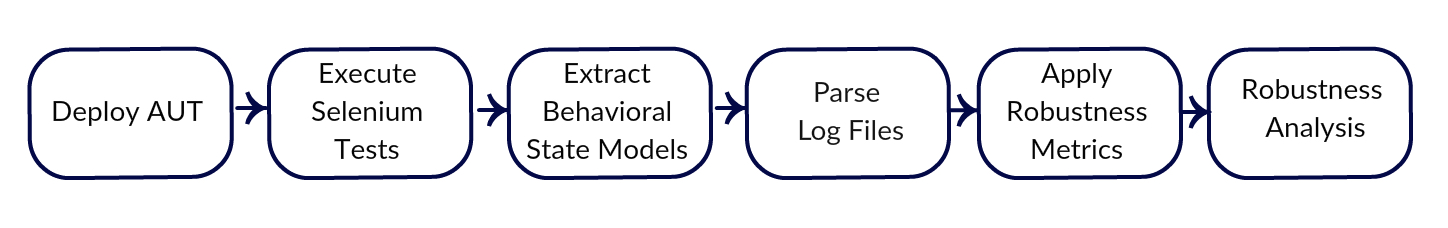
\includegraphics[width=\textwidth]{./Figures/thesisoverviewsmall.jpg}
%     [width=5cm, height=3cm]
% 		\rule{35em}{0.5pt}
	\caption{Setup required for the robustness analysis}
	\label{fig:thesisoverview2}
\end{figure} 

\subsection{Automatic application deployment}
\label{sec:autoDeployment}
% \section{Web Application Deployment}

To measure the robustness of Selenium tests across different versions of AUT, the first step of the implementation setup is to make these versions accessible for the testing setup as shown in Figure \ref{fig:thesisoverview2}. It is possible to accomplish this by installing and deploying these versions locally (without relying on external application server provider). The most common ways to release such web applications are either by releasing packaged versions ready to deploy, such as \texttt{war} (Web application ARchive) files in case of Java applications or by checking out the code from version control repositories such as git, subversion, mercurial etc.

\begin{figure}[h]
\makeatletter 
% \renewcommand{\thefigure}{\@arabic\c@figure}
\makeatother
% \setcounter{figure}{0}
    \centering
  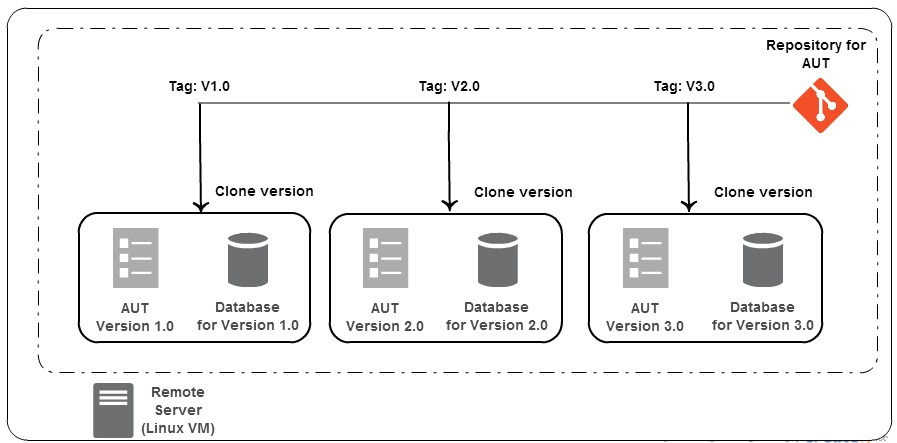
\includegraphics[width=5.4in,height=2.6in]{./Figures/Deployment_Process_2.jpg}
  \caption{Automatic parallel deployment process}
  \label{fig:deployment} 
\end{figure}

Depending upon the type of the web application as well as the frameworks and programming languages used to create these application, different set of application servers need to be used. Java based packaged applications such as \texttt{war} archives can be deployed in Java containers such as Tomcat\footnote{\url{http://tomcat.apache.org/}}. Similarly, PHP based applications can be hosted inside Apache httpd\footnote{\url{https://httpd.apache.org/}} servers. 

The AUT can be deployed as per the installation instructions provided by the application vendors. The installation setup includes steps such as downloading the application source code or packaged binaries, creating databases and other configurations etc. Certain Selenium tests require the AUT to have some pre-configured features enabled, such as an \textit{administrative} user account setup which can also be accomplished in the installation phase. 

In order to spare the manual effort of installing multiple versions of AUT, the deployment work-flow can be automated through means of deployment scripts such as automated shell scripts. To further expedite the testing process, we aim to deploy multiple versions of the AUT in parallel, sand-boxed inside a secure Linux based virtual machine for security reasons. Figure \ref{fig:deployment} depicts the overview of remote automatic deployment process; three versions of the AUT are running simultaneously against their individual database instances.

% \subsection{Automatic application deployment}
\section{Behavioral State Models}
\label{stateModelExtraction}
% \section{State mapping (RQ1)}
% \section{Feature selection (RQ2)}
% \section{Analyzing changes in test suites (RQ3)}